\documentclass[twoside,10.5pt]{article}
\usepackage{jmlr2e}
\usepackage{subfigure}
\usepackage{hyperref}
\usepackage{endnotes}
\usepackage{enumitem}
\setlength{\parskip}{0pt}
\setlength{\parsep}{0pt}
\setlength{\headsep}{5pt}
\setlength{\topskip}{0pt}
\setlength{\topmargin}{0pt}
\setlength{\topsep}{0pt}
\setlength{\partopsep}{0pt}
\let\footnote=\endnote
\renewcommand{\notesname}{Endnotes}
\newcommand{\dataset}{{\cal D}}
\newcommand{\fracpartial}[2]{\frac{\partial #1}{\partial  #2}}
\ShortHeadings{95-845: AAMLP Project}{Gangwar, Rost and Setia}
\firstpageno{1}

\begin{document}

\title{Heinz 95-845: Project Report}

\author{\name Mridul Gangwar \email mgangwar@andrew.cmu.edu \\
       \addr Heinz College of Information Systems and Public Policy\\
       Carnegie Mellon University, Pittsburgh, PA, United States \
       \AND
       \name Lauren Rost \email lrost@andrew.cmu.edu \\
       \addr Heinz College of Information Systems and Public Policy\\
       Carnegie Mellon University, Pittsburgh, PA, United States \
       \AND
       \name Nikita Setia \email nikitas@andrew.cmu.edu \\
       \addr Heinz College of Information Systems and Public Policy\\
       Carnegie Mellon University, Pittsburgh, PA, United States}
       
\maketitle
\vspace*{5px}
\begin{abstract}
Opioid overdose deaths spiked in 2017 and continue to be a major concern for the US healthcare system. Major efforts have been dedicated to understand the demographic impacted and how the healthcare system can improve outcomes for individuals at risk. This paper explores the application of machine learning and statistical analyses to identify which could best predict (and prevent) overdose deaths using county-provided demographic, program activity and opiate prescription fills data for Medicaid beneficiaries from 2009-2017. The models with superior performance, Multivariate Logistic Regression and Random Forest, yield an AUROC of approximately 0.83, correctly identifying 57\% of individuals who overdose. *Need to add a line about variable importance*. As such, this paper showcases how county-provided data can be used to predict and prevent overdoses (translatable to other counties), identifies the variables indicative of risk, and highlights modeling techniques that can be tuned to improve predictive performance, thereby moving the field towards overdose prevention.  
\end{abstract}

\section{Introduction}
Opioid abuse has been an emerging public health issue, and was declared a public health emergency in 2017\footnote{\cite{HHS}}. In the past two decades, national drug overdose deaths have increased from 16,849 in 1999 to 70,237 in 2017\footnote{\cite{NIDA_ODR}}. This trend is especially affected by the onset of the opioid epidemic in the late 1990s\footnote{\cite{NIDA_OOC}}. Approximately 67\% of the overdose deaths in 2017 were due to the involvement of any opioids (including illegal drugs like heroin and fetanyl) and 24\% are specifically due to legally prescribed opioids, like oxycodone, hydrocodone, codeine, morphine, etc.\footnote{\cite{NIDA_ODR}}\footnote{\cite{NIH_OpioidsInfo}}. It has become critical to better understand the risk factors leading to overdoses and to determine the best way to prevent overdose deaths. \\

Crosier et al. predicted overdose frequency using random forests in order to uncover important features related to the frequency and development of overdose events\footnote{\cite{Sage}}. Lobo et al. identified sub-groups of Pennsylvania patients at greater risk for opioid abuse in a k-means clustering algorithm\footnote{\cite{Lobo}}. Our work aims to contribute to this existing body of work by identifying features that are most indicative of risk, which is crucial to preventing addiction and overdoses. There exists an Opioid Risk Tool, developed in 2005, to flag patients at risk for opioid abuse and overdose\footnote{\cite{Webster}}. However, due to the subjective nature of this tool and the spike of deaths in 2017, machine learning has been sought to provide a more objective and quantitative approach to estimate risk of opioid abuse and overdose. A super learning approach was developed by Acion et al. to predict the successful treatment of patients with substance use disorders\footnote{\cite{Acion}}. Artificial intelligence was also applied in the sphere of predicting opioid abuse by Haller et al., who implemented natural language processing on electronic health record data to assess risk and predict opioid abuse\footnote{\cite{Haller}}. \\

This paper strives to expand upon previous contributions to the field by identifying the machine learning algorithms that yield the highest predictive performance of overdose events. Specifically, those models that correctly identify the greatest number of at-risk individuals. This project uses datasets containing information concerning demographics, county-provided program usage, and opioid prescriptions to predict overdose deaths (opioid and non-opioid). Specifically, we analyze the data of Medicaid beneficiaries from 2009 to 2017 provided by the Allegheny County Department of Human Services (DHS) to predict the risk of death due to an non-opioid or opioid-related overdose. Here, we apply machine learning to uncover features and methods that successfully predict overdose death, and thereby enhance the space of addiction and overdose death prevention. 

\section{Methods}
\subsection{Original Data Description}
We accessed 3 datasets from Allegheny County DHS: demographic, program activity, and opiate prescription fills. Information within contained data for 120,650 individuals who have utilized DHS services between 2009 and 2017. The demographic dataset (summarized in figure \ref{fig:orig_dem}) contained variables for person ID, race, and gender. Of note, there was missingness in terms of race data for 19,531 individuals and gender information for 210 individuals. Additionally, there were demographics that were not heavily represented in the rest of the dataset: one transgender female and 19 Native Hawaiian / Pacific Islanders. \\

The program dataset (summarized in figure \ref{fig:orig_prog}) contains 2,402,479 rows where each row denotes the activity (or activities) for an individual at any time since they entered the system. The program dataset contains variables for person ID, year and month of activity, overdose details (if any), and the DHS program-related relevant activity information. Program-related activity information included whether there was documentation for Child, Youth and Family (CYF) services used as child or parent (binary); the number of criminal court cases (drug or not) filed; mental health, drug and alcohol abuse, or prescription services (binary); and whether the individual was jailed (binary). If an individual experienced an overdose event, there were additional data fields for overdose date and a binary value for whether the overdose was opioid-related. The only missingness in the program activity dataset is in the overdose-related fields for individuals who did not overdose. As such, this missingness is important in considering the significance of our analyses. Otherwise, there is no additional missing data in the program activity dataset. \\

The opiate prescription fills dataset (summarized in figure \ref{fig:orig_presc}) contains 1,161,650 rows, where each row represents a prescription fill for an individual. The prescription information variables are the claim number (unique for each row), person ID, age at prescription, dispensed quantity, days supply, fill date, and information specific to the drug (drug strength, name variations, package description, and dosage form). We did not include generic tier description and claim rank of prescriptions in our analyses for they are not informative. There were missing, extreme or incomprehensible values in the prescription dataset, such as an age of -7990, dispensed quantity of 17936 and days supply of 907. In addition, the prescription dataset contained three columns of  multiple versions of drug names for the same drug. There were two columns pertaining to the drug dosage form, a condensed version and a descriptive version.

\subsection{Data Cleaning and Feature Extraction}
\subsubsection{Demographic and Program Datasets}
The missing race and gender information in the demographic dataset is likely missing not at random (MNAR) as it may be directly related to the unreported value itself. We dealt with this missingness through assigning missing values their own category, "No Data". Furthermore, with respect to the race column, given that the "Native Hawaiian / Pacific Islander" demographic was underrepresented with only 19 individuals, we merged these individuals with the "No Data" race category to create a variable called "No Data and Other". This was replicated for the gender variable where we merged the "Transgendered male to female" and the "No Data" categories into "No Data and Other." With respect to the program activity dataset, we cleaned the outcome variable by converting the 0, 1 and NA to "Non-Opiate Overdose", "Opiate Overdose" and "No Overdose". 

\subsubsection{Opiate Prescription Fills Dataset}
The data cleaning tasks performed on this dataset were as follows: First, the age at which an individual got their first prescription (entered the dataset) was extracted. If the minimum age was less than 0, the maximum age was used. If both values were less than 0, then they were considered missing. There were 26 individuals with missing age values; these were replaced with the median age of individuals in the entire dataset. Next, drug strength values of oral solutions were updated to 5-325/5ML and of Naloxone were updated to 50MG-0.5MG. Next, days supply and dispensed quantity extreme values were censored. The top extreme values were replaced with the value at the 0.5\% percentile and bottom extreme with the value at the 95.5\% percentile. These percentile values were determined for each generic name and dosage form combination. Then, opioid strength values were pulled from the drug's label name, normalized to be per 1 ML, MCG or MG (if applicable). Missing values were replaced with those from provided drug strength column. Next, we obtained Opioid Morphine Equivalent Conversion Factors\footnote{\cite{CMS}} to convert the above-mentioned opioid strength values into Morphine Milligram Equivalent (MME). The formula used is: $opioid\,strength * (dispensed\,quantity / days\,supply) * conversion\,factor$
Last, drug name (generic) and dosage forms were stripped to common terminology. An example is changing Oxycodone HCL to Oxycodone for drug name and combining Tablet and Capsule to Pill in dosage form. 

\subsubsection{Final Dataset}
There were 30 meaningful features that were extracted at the person ID level regarding each individual's demographic characteristics, their participation in DHS program activities, and their opiate prescription fills. Demographic characteristic features included race, gender and age. DHS program usage features entailed cohort (the enrollment year in DHS services), usage of CYF program as child ($total\_cyfchild$) and as parent ($total\_cyfparent$), use of mental health, drug and alcohol abuse and prescription services ($total\_mh$, $total\_da$, $total\_rx$), number of months spent in jail ($total\_acj$), and number of criminal cases ($total\_cr\_cases$) and drug-related cases filed in court ($total\_cr\_drug\_cases$). \\

Prescription activity features extracted included the number of prescriptions ($num\_presc$), name of the most prescribed drug ($most\_presc\_drug$) and most prescribed dosage form ($most\_dose\_form$), count of top three drugs ($oxy\_count$, $tram\_count$, $hydrobit\_count$), count of top three dose forms ($pill\_count$, $patch\_count$, $liquid\_count$), average, median and mode MME ($avg\_mme$, $median\_mme$, $mode\_mme$), as well as average days supply and dispensed quantity ($avg\_supply$ and $avg\_dispensed$). Finally, overdose information ($od\_type$, $od\_month$, $od\_year$, $od\_date$) was added. 

\subsubsection{Feature Choices}
Some additional feature choices were made to enhance the final dataset and prepare for the prediction tasks. Features such as $most\_presc\_drug$ and $most\_dose\_form$ had categories that were comprised of less than 0.2\% of the values. To prevent errors during the prediction task, these low occurrence categories were combined to create a separate “Other” category. We plotted the distribution of the average, median, and mode of morphine milligram equivalents (MME) variables to determine which mode of central tendency for MME was normally distributed. This led us to retain only median MME in the final dataset to avoid multicollinearity.\\

We examined the outcome variable under a binary value of 1 for an "opiate overdose" or "non-opiate overdose" and 0 for there being "no overdose". "Non-opiate overdose" represents a situation for which there were no opioids found in the individual's system upon an overdose death. We include these events in our outcome variable due to the fact that these individuals were receiving opioid prescriptions, so in an effort to flag as many individuals as possible from dying from opioid overdose, we are willing to increase the number of potential false positives in being more inclusive in our outcome variable. Furthermore, we argue that individuals who overdose (opiate or non-opiate) share similar characteristics and so the inclusion of both types of overdose in our outcome variable is informative in the prediction task.Columns pertaining to the date of overdose were removed to avoid leakage in the machine learning models, as they are proxies for the target variable. All categorical variables were converted to dummy variables. We applied a log transformation to all feature variables. 

\subsection{Oversampling, Machine Learning and Statistical Models, and Evaluation Metrics}
Since there is a severe under-representation of outcome variable events (1,222 out of 120,650 individuals), the first model (multivariate logistic regression) was unable to capture a single case of overdose. As such, this paper utilized an oversampling method, Synthetic Minority Oversampling Technique (SMOTE) for the outcome variable. To do so, we divided the whole dataset into train and test with a 50-50\% split. We then ran SMOTE on the train set to generate synthetic data to train our models and then calculated performance on the original test set. Furthermore, to increase the performance of our machine learning models, we trained the data only on the top 20 critical features identified using the random forest algorithm.\\

Six machine learning models were run and their performance in predicting overdose rates compared. These models include: multivariate logistic regression, ridge regression, random forest, AdaBoost, gradient boosting, and neural nets. We used 5-fold cross-validation for multivariate logistic regression, and 10-fold cross-validation for ridge regression, random forest, and gradient boosting. We also implemented lasso regularization. Note that for this use case in particular, it is more critical to identify the individuals who may overdose (true positives) than to eliminate individuals not at risk from consideration (true negatives). Furthermore, given the limited resources available to tackle such a pressing issue, it is valuable to minimize (to the extent possible) the number of individuals incorrectly identified to be at risk (false positives). Therefore, we evaluated and compared machine learning models through the area under the curve (AUC) of the Receiver Operating Characteristic (ROC) curves, the number of true positives, the number of false positives, sensitivity, specificity, and precision. The important or significant features used in these models will also be an additional point of comparison, specifically for the multivariate logistic regression and random forest models.\\

This paper also includes a survival analysis, conducted using Kaplan-Meier estimation and Cox Proportional Hazards models. For the survival analysis, the time variable was the months in system and the event variable was the status of the individual at their last known month in the system. The event was 1 for overdose death and 0 otherwise. The Kaplan-Meier estimation was evaluated visually (with the survival curve) along with the model output. Both normal and regularized versions of the Cox Model were produced. The coefficients, exponent coefficients and their corresponding p-values were used to understand and evaluate both models. Cross-validation was used to determine the best lambda to use for the regularized Cox Model. 
Code is available at https://github.com/nikitascmu/S19-aamlp-project-group1. 

\section{Results}

Table \ref{tab:table1} provides an overview of the 120,650 individuals in the Allegheny County DHS cohort between 2009 and 2017. No individuals were excluded from the cohort. We addressed all missingness to the extent possible.

\begin{table}[h!]
  \begin{center}
    \caption{Demographics of Allegheny County DHS Cohort (2009-2017).}
    \label{tab:table1}
    \scalebox{0.7}{
    \begin{tabular}{l|c|r}
      \textbf{Characteristic} & \textbf{N} & \textbf{Percentage (\%)}\\
      \hline
      $Race$ & $ $ & $ $ \\
      White & 56,754 & 47.04\\
      Black/African-American & 40,573 & 33.63\\
      Biracial/Multiracial & 2,118 & 1.75\\
      Asian & 1,216 & 1.00\\
      American Indian/Alaskan Native & 439 & 0.36\\
      No Data and Other & 19,550 & 16.20\\
      \textbf{Total} & \textbf{120,650} & \textbf{100}\\
      \hline
      $Gender$ & $ $ & $ $ \\
      Female & 73,582 & 60.99\\
      Male & 46,857 & 38.84\\
      No Data and Other & 211 & 0.17\\
      \textbf{Total} & \textbf{120,650} & \textbf{100}\\
      \hline
      $Age (years)$ & $ $ & $ $\\
      0-19 & 27,128 & 22.48\\
      20-39 & 51,883 & 43.00\\
      40-59 & 35,941 &  29.79\\
      60 \& Over & 5,698 &   4.72\\
      \textbf{Total} & \textbf{120,650} & \textbf{100}\\
      \hline
    \end{tabular}}
  \end{center}
\end{table}

\subsection{Evaluation of Machine Learning Models}
The ROC curves of all 6 machine learning models run in this paper are showcased in figure \ref{fig:auc_curves} below.  

\begin{figure}[htp]
\centering
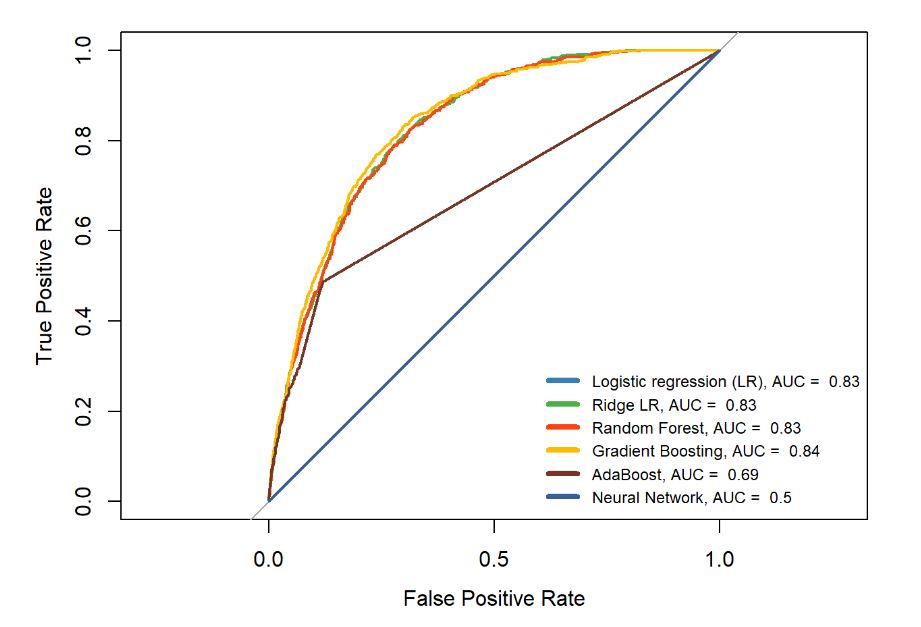
\includegraphics[width=10cm]{images/auc_curves.JPG}
\caption{Receiver Operating Characteristic (ROC) curves with corresponding AUCs for the 6 ML models}
\label{fig:auc_curves}
\end{figure}

These curves, along with their reported AUCs, indicate that Gradient Boosting performs the best with Logistic Regression, Ridge Regression, Random Forest close behind. AdaBoost does not perform well and Neural Networks perform only as good as chance. As such, AdaBoost and Neural Networks can be dropped from consideration for the time being. However, it would be premature to select Gradient Boosting as the best model. As stated earlier, it is vital to identify the individuals who are at risk of overdose (true positives) while keeping the number of false identifications to a minimum. As such, while Gradient Boosting may appear to perform the best, whether it is truly the best model in this case depends on its performance on additional evaluation metrics. 

\begin{table}[h!]
  \begin{center}
    \caption{Evaluation Metrics of the Machine Learning Models}
    \label{tab:metrics}
    \scalebox{0.7}{
    \begin{tabular}{l|c|c|c|c|c|c}
      \textbf{Model} & \textbf{True Positives} & \textbf{False Positives} & \textbf{Sensitivity (\%)} & \textbf{Specificity (\%)} & \textbf{Precision (\%)} & \textbf{AUC}\\
      \hline
      Multivariate Logistic Regression & 362 & 8654 & 57 & 86 & 4 & 0.83\\
      Ridge Regression & 163 & 2422 & 26 & 96 & 6 & 0.83\\
      Random Forest & 362 & 8654 & 57 & 86 & 4 & 0.83\\
      Gradient Boosting & 138 & 1982 & 22 & 97 & 7 & 0.84\\
      Ada Boost & 147 & 2389 & 23 & 96 & 6 & 0.69\\
      Neural Net & 633 & 59692 & 100 & 0 & 0 & 0.5\\
      \hline
    \end{tabular}}
  \end{center}
\end{table}

Table \ref{tab:metrics} summarizes the performance of all six machine learning models in predicting overdose deaths. Please note that there are 633 overdoses in the test dataset. As seen in this table, despite having the highest AUC, Gradient Boosting correctly identifies only 22\% of overdose deaths (few relative to the other high performing models). Neural nets identifies all overdose deaths simply because it classifies every individual at risk of overdose, so it can be excluded from consideration. Of the remaining four models, Multivariate Logistic Regression and Random Forest perform the best, correctly identifying 57\% of the at-risk individuals. 

\subsection{Understanding the Survival Analysis}
Survival analysis using the Kaplan-Meier estimation yields a median survival of 110 months in system. This can be seen in the survival curve in figure \ref{fig:km_original} in the appendix. A slight decline in the probability of survival can only be seen after an individual has been in the system for over 90 months (7.5 years). We can also see that individuals have dropped out of the system throughout the time-frame. However, 

\begin{figure}[h!]
\centering
\begin{minipage}{.5\textwidth}
  \centering
  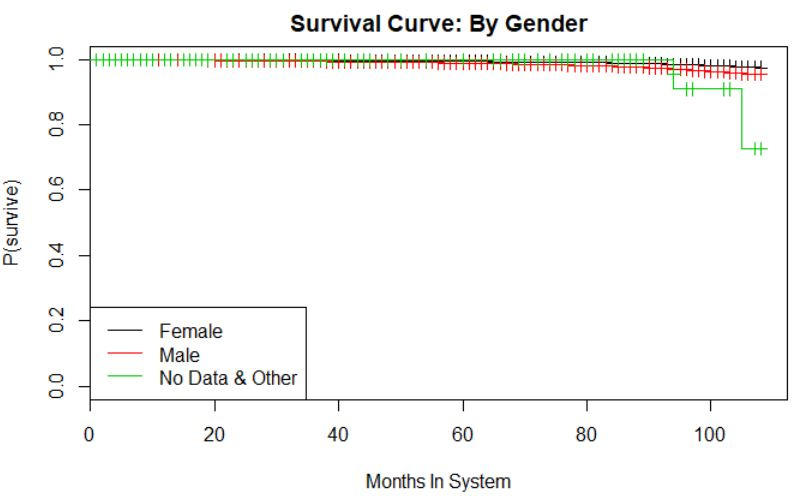
\includegraphics[width=1\linewidth]{images/kaplan_meier_gender.JPG}
  \caption{Kaplan Meier curve by gender indicates a lower probability for survival for individuals in the "No Data and Other" category, and also slightly lower probability of survival for men, as compared to women.}
  \label{fig:km_gender}
\end{minipage}%
\begin{minipage}{.5\textwidth}
  \centering
  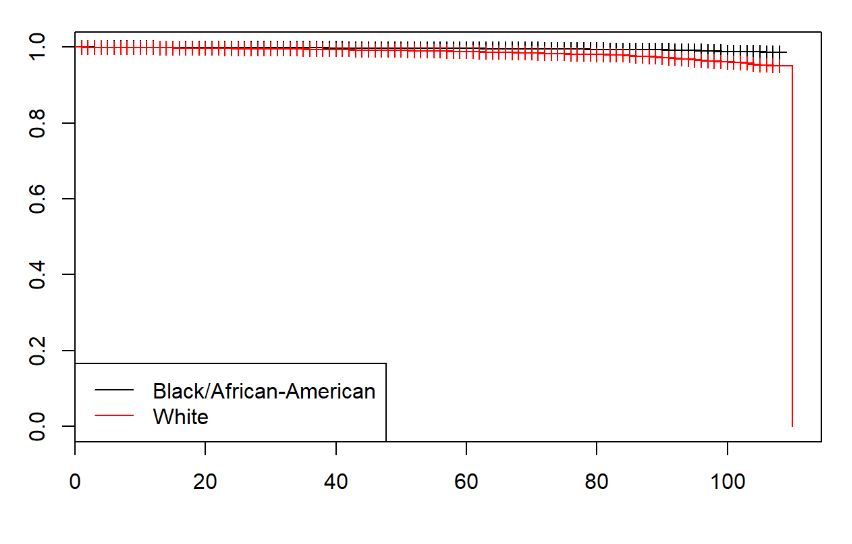
\includegraphics[width=1\linewidth]{images/kaplan_meier_race.JPG}
  \caption{Kaplan Meier curve by race indicates a lower probability for survival for white individuals, as compared to Black / African-American individuals.}
  \label{fig:km_race}
\end{minipage}
\end{figure}



\subsection{Variable Importance}
We found that the most informative variables to opioid overdose was the total number of Tramadol prescribed(tram\_count), the total number of drug and alcohol services received(total\_da), being of white race(race\_White), the total number of lower court drug-related criminal cases(total\_cr\_drug\_cases), being of the male (gender\_Male) or female(gender\_Female) gender, median number of MME (median\_mme), total number of mental health service records of services

\begin{figure}[h!]
\centering
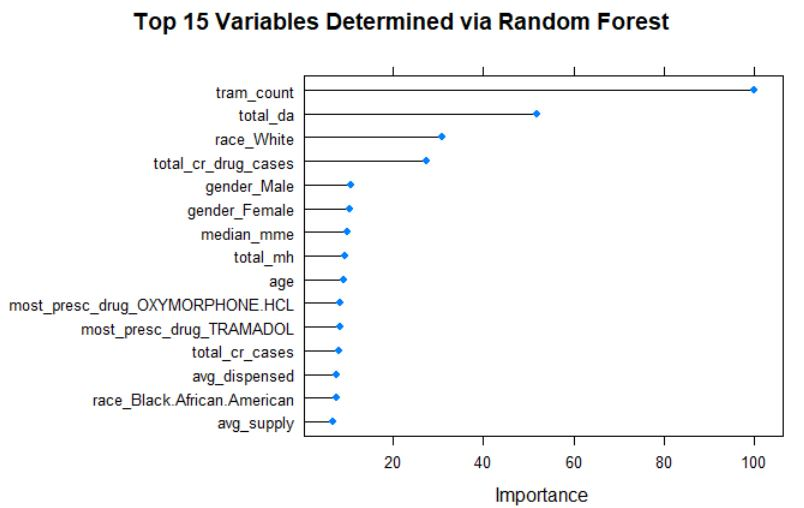
\includegraphics[width=12cm]{images/variable_importance.JPG}
\caption{Variable Importance... }
\label{fig:var_importance}
\end{figure}



\section{Discussion}
Our machine learning models yielded low sensitivity, and fairly high specificity. With low sensitivity, we are getting a lot of false negatives and few true positives, however for our context and our intended application of these machine learning models, this could be beneficial in being extra cautious with individuals who are predicted to be at risk for an opioid overdose death. However, the low sensitivity may overburden counties' department of health services, which may lead to a completely impractical alogrithm, and thus it may have no actual impact on preventing opioid overdose death. Precision was very low, which may be due to the few number of opioid and non-opioid overdose events in our dataset.\\ 
Another reason that our machine learning algorithms are not performing well is that we were not able to tune the hyperparameters, which we would expect to have a significant impact on performance. The neural network had such poor performance due to the fact that we used only four dense layers and ran the algorithm for 30 epochs. We would expect that a deep neural network with a large number of layers running for a large number of epochs would perform better, however we were computationally under-powered to implement such a technique. \\
There are limitations to our work in that our algorithm may not be generalizeable to other county health systems, especially if they do not collect our selected similar data fields. Our study is also limited by the fact that we do not have other potentially relevant data fields that may be informative to understanding opioid overdose death, like socioeconomic status, medical history, diagnoses, and insurance claims. \\


\section{Conclusion}
In implementing appropriate data cleaning and feature selection, we were able to apply a machine learning model with sufficient predictive power to perhaps be of use to a county health department to predict opioid overdose death. In moving forward, we suggest applying a dataset that is more enriched for opioid overdose deaths outcomes to our machine learning pipeline in order to more accurately flag people at risk for opioid overdose death. In addition, in order to truly understand the impact of this work on predicting opioid overdose death, one would have to see how the implementation of this pipeline in a real-world setting would perform. This study would demonstrate the actual practicality and use of utilizing the risk prediction tool in a county department health service setting.\\

how county-provided data can be used to predict and prevent overdoses (translatable to other counties), identifies the variables indicative of risk, and highlights modeling techniques that can be tuned to improve predictive performance, thereby taking a giant step towards overdose prevention. 

\newpage
\appendix
\section*{Appendix}
We also performed a correlation analysis to better understand the relationship between numerical variables. During the exploration we found out some interesting relationship like hydrobit count is positively correlated with total Rx, number of prescriptions, and pill count.

\begin{figure}
\begin{center}
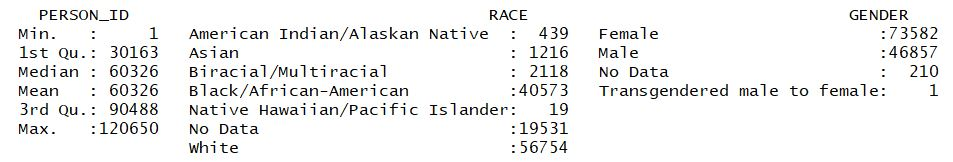
\includegraphics[width=5in]{images/original_dem_summary.JPG}
\end{center}
\caption{Summary of the original demographic dataset.}
\label{fig:orig_dem}
\end{figure}

\begin{figure}
\begin{center}
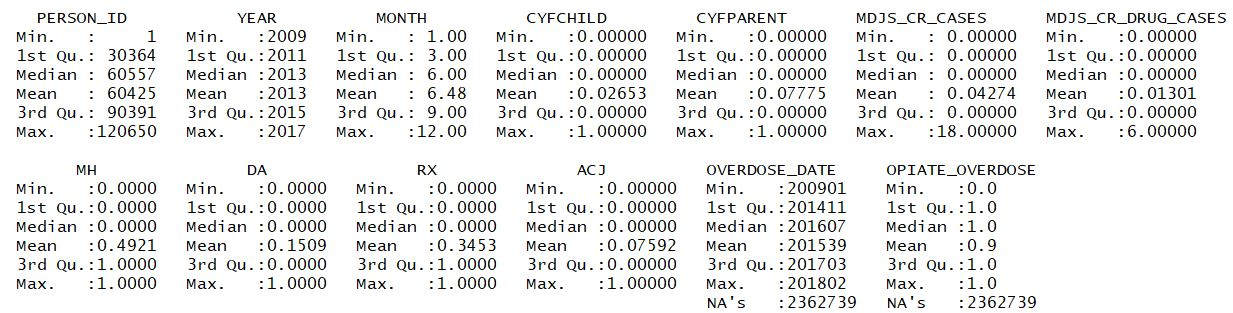
\includegraphics[width=6in]{images/original_prog_summary.JPG}
\end{center}
\caption{Summary of the original program activity dataset.}
\label{fig:orig_prog}
\end{figure}

\begin{figure}
\begin{center}
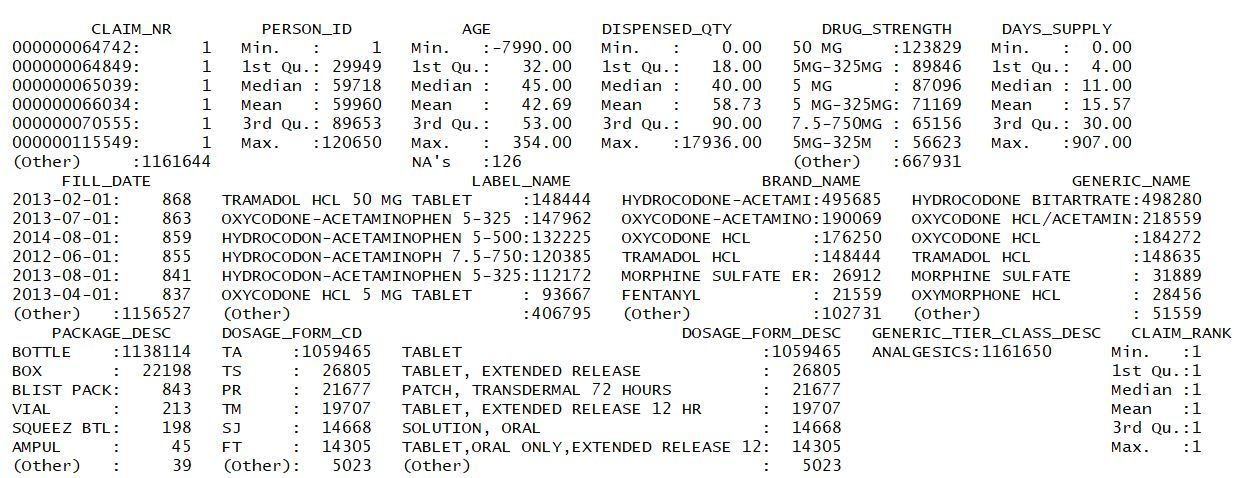
\includegraphics[width=6in]{images/original_presc_summary.JPG}
\end{center}
\caption{Summary of the original opiate prescription fills dataset.}
\label{fig:orig_presc}
\end{figure}

\begin{figure}[htp]
\centering
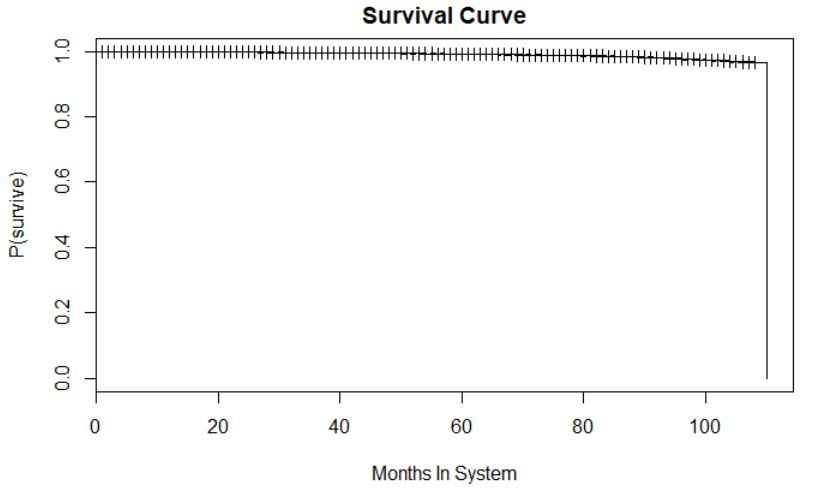
\includegraphics[width=12cm]{images/kaplan_meier.JPG}
\caption{Kaplan Meier curve of survival indicates that }
\label{fig:km_original}
\end{figure}

\newpage
\theendnotes
\bibliographystyle{ieeetr}
\bibliography{final_bibliography.bib}



\end{document} 
